\chapter{Supervised Progressive Autonomous Robot Competencies}\label{chap:sparc}

\begin{framed}
	\textbf{Key points:}
	
	\begin{itemize}
		\item Novel interaction framework to teach robots an action policy while interacting
		\item Provides the human teacher control on the robot actions whilst the robot learns from this supervision
		\item Teacher provide feedback on intention rather than action
		\item The robot behaviour (under supervision) can be assumed to be optimal
		\item Reduces workload on the teacher over time as the robot learns
	\end{itemize}
\end{framed}

Parts of the work presented in this chapter have been published in \cite{senft2015sparc} and \cite{senft2017supervised}. The final publications are available from Springer and Elsevier via \url{http://dx.doi.org/10.1007/978-3-319-25554-5_60} and \url{https://doi.org/10.1016/j.patrec.2017.03.015}.

\newpage

As presented in Chapter \ref{chap:background}, robots would profit from being able to learn from humans how to interact with other humans. Using \gls{iml} to achieve this transfer of social and task knowledge from the human domain-expert to the robot would result in a faster approach than slow iterative update of behaviour by engineering an action policy or learning by trials and errors as with \gls{rl}.

However, as stated in that chapter, \gls{iml} is seldom applied to learning to interact with humans and no current system provide the teacher with enough control over the robot action to ensure that the first principle presented in Section \ref{ssec:back_constraints} (``Only execute appropriate actions'') is validated. Techniques relying solely on feedback cannot prevent the robot to execute an incorrect action, but only reward negatively incorrect actions after their execution \citep{senft2017supervised} and techniques based on \gls{lfd} do not learn an action policy online providing the desired adaptivity in time of behaviour.

In order to provide a robot with an appropriate action policy, adaptive to different context or behaviours and requiring a low workload on the teacher or supervisor, we introduce in \cite{senft2015sparc} the \acrfull{sparc} framework of interaction to allow end-users to safely teach a robot an action policy.

\section{Principles} \label{sec:sparc_principles}

\gls{sparc} defines an interaction between a learner and a teacher following these principles:
\begin{itemize}
	\item The learner has access to a representation of the state and a set of actions
	\item The teacher can select actions for the robot to do.
	\item The learner can propose actions to the teacher
	\item The teacher can enforce or cancel actions proposed by the learner and actions non evaluated are executed after a small delay
	\item The learner improves its action policy using the teacher's commands and feedback on propositions
\end{itemize} 

This way of keeping a human in the loop and in control of the robot's actions is equivalent to the level 6 on the Sheridan scale of autonomy: "A computer selects action, informs human in plenty of time to stop it" \citep{sheridan1978human}. In addition, a learning algorithm improve the correctness of suggested actions decreasing the probability of requiring the teacher to correct actions or having to select new actions. Additionally, keeping the human in the loop also allows them to provide additional information to the algorithm to speed up the learning.

This approach can be compared to predictive texting as seen on phone nowadays. The user can select the words proposed by the algorithms, or write their own, and the algorithm learns the user's preferences and habits and aims to suggest words more and more appropriate to the user. However, \gls{sparc} enables a more complex interaction between learner and teacher and is directed to interactive environments where the context changes with time both dependently and independently to the agent actions.

\section{Goal}

The goal of \gls{sparc} is to allow non-experts in computer science to teach quickly an action policy to a robot by guiding its interaction with an environment, without requiring constant input from a human whilst ensuring that the robot's behaviour is constantly appropriate. 

Figure \ref{fig:concept} presents an idealist comparison of the expected workload, performance and autonomy of three methods: autonomous learning (such as \gls{rl} - \citealt{sutton1998reinforcement}), feedback based teaching (such as TAMER - \citealt{knox2009interactively}) and \gls{sparc}. Unlike other methods, by following the principles presented in the previous section, \gls{sparc} is expected to maintain a constant high performance even during early stages of learning, and to see a decrease of workload on human supervisor as the agent improve its action policy using machine learning and the suggestions become more accurate.

%TODO: could add woz
\begin{figure}[ht]
	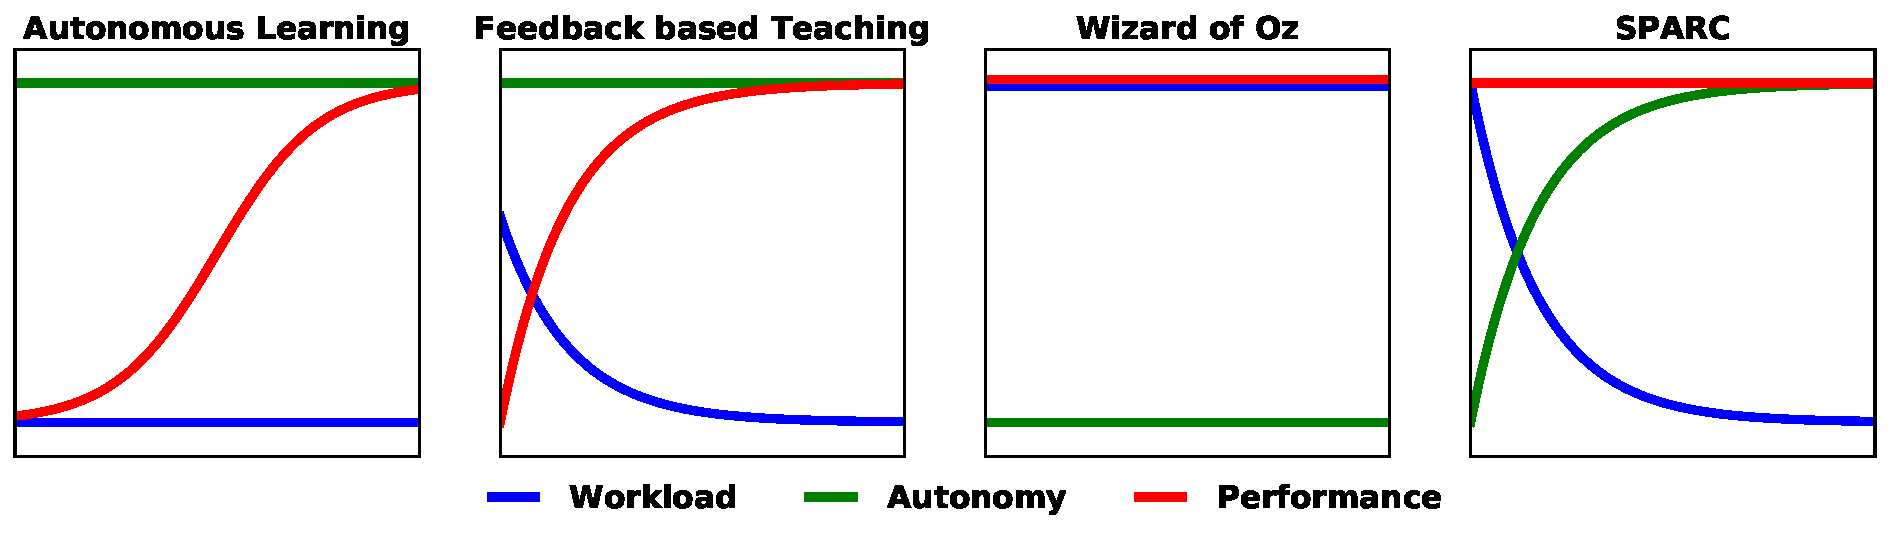
\includegraphics[width=.8\linewidth]{concept.pdf}
	\centering
	\caption{Idealistic comparison between autonomous learning, feedback base teaching and \gls{sparc}.}
	\label{fig:concept}
\end{figure}

Once the behaviour is deemed appropriate enough by the teacher, the agent can be deployed to interact autonomously in the real world if this output is desired. Alternatively, in context where a human expert cannot be removed from the control loop, such as \acrlong{rat}, the supervisor can stay in control of the robot actions in a supervised autonomous way (level 6 of Sheridan) and only intervene when the agent is about to do an error. This approach is similar to safety drivers behind autonomous vehicles but with information about the car's intentions rather than solely the car's actions. 

\section{Frame}

Similarly to other applications of \gls{iml}, SPARC requires the interaction with a teacher to learn an action policy to interact with the world. In this framework, the robot interacts with two entities: the target and the teacher, which results into two interlinked interactions: the application interaction (task the robot learns to achieve) and the control interaction (relation with the teacher), as demonstrated in Figure \ref{fig:frame}. In the generic case, the general interaction is a triadic interaction (Teacher-Robot-Human target), such as a teacher teaching a robot tutor how to support child learning (as implemented in Chapter \ref{chap:education}). But in specific cases, the overall interaction can be only dyadic (Teacher-Robot-Teacher or Teacher-Robot-Environment), such as  robot at home learning from its user how to support them better.

\begin{figure}[ht]
	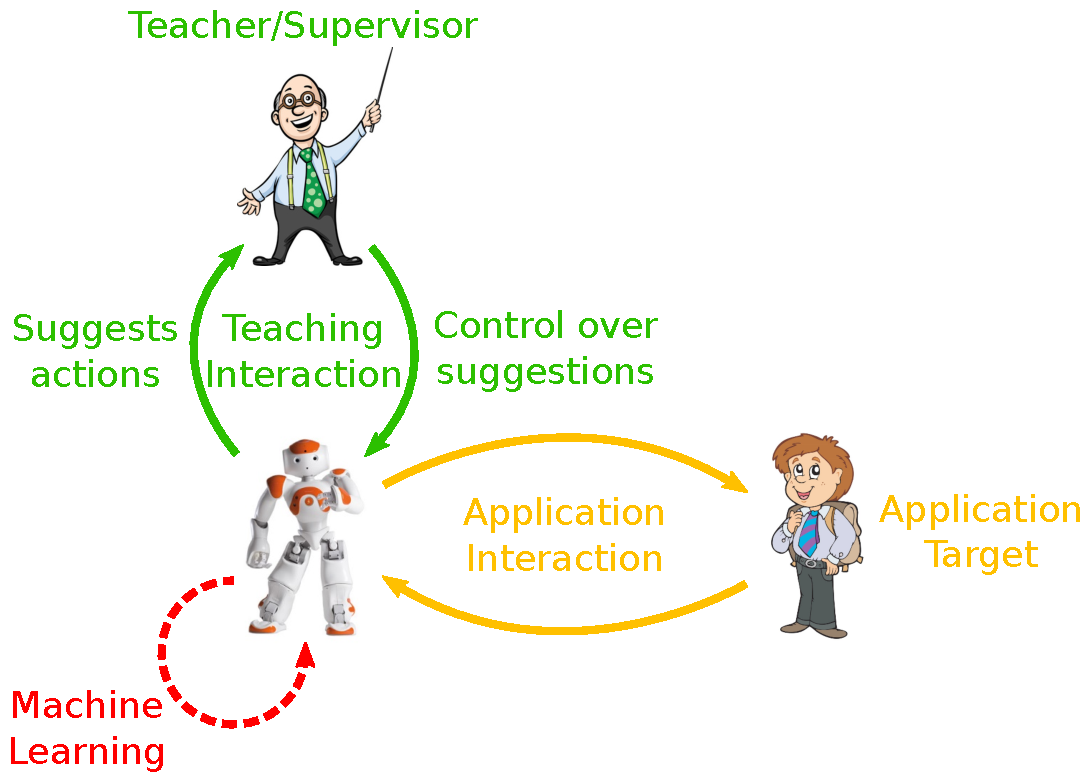
\includegraphics[width=.8\linewidth]{frame.pdf}
	\centering
	\caption{Frame of the interaction: a robot interact with a target and suggests actions and receive commands from a teacher.}
	\label{fig:frame}
\end{figure}

However, unlike some other \gls{iml} approaches, the requirement of a human in the action selection loop limits the timescale of interaction. As the human has to be provided with few seconds to react to the proposition, the rate of actions has to be 0.5 Hz or below. However, this can be mitigated by using higher level actions and this has the advantage to ensure that only correct actions will be executed without requiring the human to select them all.

\gls{sparc} presents many similarities with \acrlong{lfd} (cf. Section \ref{ssec:back_lfd}) as it uses human demonstration of policies to learn. However, most of the applications of \gls{lfd} \citep{argall2009survey,billard2008robot} are focused on learning a manipulation skill in a mostly deterministic environment. \gls{lfd} has seldom been used to teach an action policy to interact with humans \citep{liu2014train,sequeira2016discovering} and never in an online fashion.

Additionally, \gls{sparc} differs from Active Leaning (cf. Section \ref{ssec:back_active}) by the fact that the agent cannot decide which sample will be evaluated by the supervisor. As the robot interacts with humans, the datapoints provided to the teacher for \textit{labelling} will emerge from the interaction, and cannot be selected at will. 
    
\section{Implications}

The principles described in section \ref{sec:sparc_principles} have also implications on the interactions between the teacher and the agent and between the agent and the environment.

As the teacher can evaluate the actions proposed by the agent before their executions, it actually evaluates the intentions of the agent rather than its behaviour, and this difference is key as traditional \gls{iml} approaches only evaluate the actions or their effects, but not the intentions. This implication is fundamental in \gls{hri} as we cannot accept to have a robot executing non appropriate actions when interacting with humans (cf. first principle in Section \ref{ssec:back_constraints}) and correctly evaluating intentions and not actions gives the opportunity to the teacher to pre-empt incorrect actions preventing the execution of undesired behaviours.

Most importantly, the control given to the teacher on the agent's actions ensures that every action executed by the in the world has been either actively or passively validated by the teacher. This implies that each action executed can be assumed to be appropriate to the current state, potentially simplifying the learning algorithm.

\section{Interaction with Machine Learning Algorithms}

The principles of \gls{sparc} define it at the crossing between \acrlong{sl} and \acrlong{rl}. The  goal of the algorithm could be either to reproduce the teacher's policy, in a supervised way or to explore using the teacher's commands and control the environment and infer an action policy in a reinforced way.

As such, \gls{sparc} only defines an interaction framework between a teacher and a learner, and it is agnostic to the algorithms: it can be combined with any algorithm used in \acrlong{sl} or \acrlong{rl}. This research explored a combination with three types of algorithms: supervised learning using feed-forward neural networks in Chapter \ref{chap:woz}, reinforcement learning in Chapter \ref{chap:control} and supervised learning using instance based algorithm in Chapter \ref{chap:education}. However \gls{sparc} could be combined with a wide range of other algorithms.

In theory, if using a reinforcement learning approach and other types of algorithms, \gls{sparc} could even go beyond the demonstrated action policy and achieve a performance higher than the demonstration as it has been demonstrated for other approaches in Section \ref{sec:back_iml}. But this has not been evaluated in this work.

\section{Summary}
    
This chapter introduced \acrfull{sparc}, a novel interaction framework to teach agent an action policy. This approach is suitable to teach a robot to interact with humans as it validates the principles defined in Section \ref{ssec:back_constraints}. \gls{sparc} starts in a similar fashion than \gls{woz}: the teacher can select which action the robot should do, then using a learning algorithm, the learner proposes actions to the teacher who can let them be executed after a short time or cancel the action and select another one if appropriate. This suggestions/corrections mechanism provides the appropriateness of actions as a human could have cancel any inappropriate action in the learning phase, provides the adaptivity as the teacher can extend the behaviour beyond the current action policy. The learning algorithm with the auto-executions ensure that once the robot has learnt the human workload is low and the robot could even be deployed to interact autonomously if this is desired.

